
\section{Exercise 8}

In this section we will explain how we developed the PCB that made
the sensor HC-SR04 work using only digital electronics. 

\begin{figure}[H]
\begin{centering}
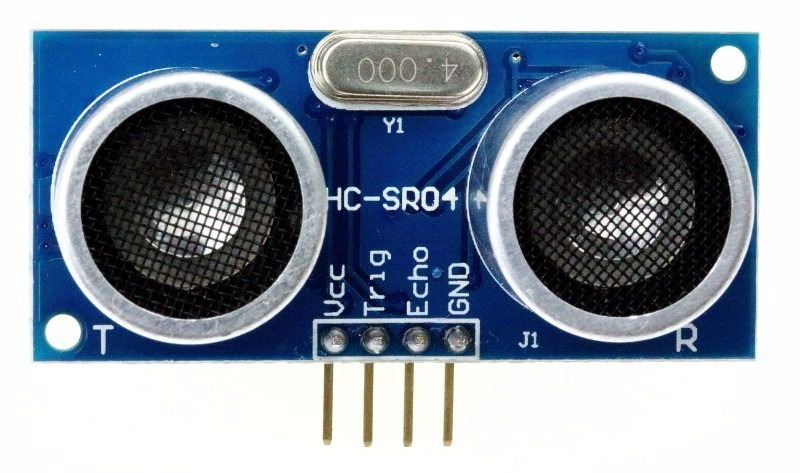
\includegraphics[scale=0.2]{images/HC-SR04}
\par\end{centering}
\caption{Sensor HC-SR04}
\end{figure}

First of all we have to explain how that sensor works.

\subsection{Sensor Operation}

This sensor has 4 pins, 2 for supply voltage (VCC and GND), and another
pair for control, these are 'Trig' and 'Echo'. The operation of this
sensor is pretty simple, you have to send a pulse of time greater
than $10\mu S$ and after some time, it will return into pin Echo,
a response pulse of duration that we will call \emph{T}. If we find
a method to measure the time \emph{T}, we can calculate the distance
measured with the following formula.

\[
Distance=\frac{T}{58}
\]

Its important to know that the time \emph{T }has to be in units of
$\mu S$ for the formula to work properly, and \emph{Distance }is
in centimeters.

A diagram of this can be found in Figure \ref{8_2}

\begin{figure}[H]
\begin{centering}
\includegraphics[scale=0.7]{\string"images/SENSOR DIAGRAM\string".eps}
\par\end{centering}
\caption{Sensor Input and output}
\label{8_2}

\end{figure}

\subsection{Components used for this Printed Circuit Board}

For this development we utilized the following Integrated Circuits
and components:
\begin{itemize}
\item 74HC4040 Counter 
\item 74HC74 D-type flip-flop
\item Two 74HC00 NAND gates
\item Two NE555 Precision Timers
\item Seven Capacitors
\item Sixteen Resistors
\item Two Diodes
\item Eight Light Emitting Diodes
\end{itemize}
The disposition of this elements in the PCB will be explained as we
undertand how we made this work.

\subsection{PCB Operation}

To make this happen, we develop this board that roughly operates as
shown in Figure \ref{8_3}

\begin{figure}[H]
\begin{centering}
\includegraphics[scale=0.5]{\string"images/Diagrama a gran escala\string".eps}
\par\end{centering}
\caption{PCB diagram}

\label{8_3}
\end{figure}

First, we have a No-Retrigger System (NRS) that filters all the retriggered
pulses we have because of buttons, that can make our board function
in an unnapropiate way. Then we generate a $50\mu S$ pulse with the
pulse generator, to send to the Trig pin of the sensor. Once we have
the respone of the sensor, we connect the Echo pin with the counter
and the measure ready logic. And finally, we plug a visual output
to the counter to see the measurement we have made. Every module seen
on this diagram, is powered by a $10kHz$ clock.

\subsubsection{No-Retrigger System operation}

This system is powered by a 74HC74 D-type flip flop that with the
proper connections we've changed it to an asynchronous SR Flip-Flop(SRFF).
To make this, we connected the SRFF pins as follows:

\begin{figure}[H]
\begin{centering}
\includegraphics[scale=0.5]{\string"images/NO-RETRIGGER SYSTEM\string".eps}
\par\end{centering}
\caption{No-Retrigger System Connections}

\end{figure}

By making this connections we made a feedback with the Q and D pins
so by every positive-edge clock Q is maintained to its previous value,
unless RESET is on. So, summarizing, by connecting the INPUT pin to
the input button, and the RESET pin to the reset button, we've created
a No-Retrigger System for our board.

\subsubsection{50 Microseconds Pulse Generator}

Making this pulse generator was a challenge, but we achieved it by
creating two submodules into the $50\mu S$ Pulse Generator Module,
these are the differentiator circuit, and the pulse generator circuit.
Tough the Differentiator Circuit is placed before the Pulse Generator
Circuit (PGC), we will explain first the PGC to better understand
the utility of the Differentiator.

\paragraph{Pulse Generator Circuit}

To power this pulse generator we've used a NE555 Precision Timer,
that by connecting it as shown in Figure \ref{8_5}, we have made
a Pulse generator of the timme we wanted.

The formula to obtain the Pulse time at the output is the following

\[
T=ln(3)C3.R2
\]

But there is a problem, this pulse generator only works if the input
pulse time is less than the time calculated on the previous formula.
So if we have a pulse generated by a human that is oviously greater
than $50\mu S$ we need a way to make this still work. So here is
were the Differentiator Circuit comes to help.

\paragraph{Differentiator Circuit}

This circuit basically differentiates an input, for us, this means
that whenever a pulse its made, a set of dirac's deltas comes out
of the circuit, one positive, and another negative. If we define $\tau$
as 

\[
\tau=RC
\]
 and we choose the apropiate values to the resistor and capacitor
to make $5\tau\leq50\mu S$ we can have a really good differentiator
circuit that for every input pulse, it creates an output of less than
$50\mu S$, and we can make work our Pulse Generator.

\begin{figure}[H]
\begin{centering}
\includegraphics[scale=0.2]{\string"images/PULSE GENERATOR\string".eps}
\par\end{centering}
\caption{Pulse Generator}
\label{8_5}
\end{figure}

\subsubsection{Measure Ready Logic}

The measure ready logic is powered by a 74HC74 D-type flip flop used
equally as the No-Retrigges System, and a differentiator circuit almost
as equal as the Pulse generator differentiator circuit. But it has
one little difference, the 74HC74 is very sensitive to negative voltage,
and it can stop working properly according to its datasheet, so we
had to add a little protection to erase the negative delta provided
by the differentiator circuit. We made this by simply adding a diode
that cancels that delta. So the circuit became as shown in the Figure
\ref{8_6}

\begin{figure}[H]
\begin{centering}
\includegraphics[scale=0.5]{\string"images/MEASURE READY\string".eps}
\par\end{centering}
\caption{Measure Ready Logic}

\label{8_6}
\end{figure}

\subsubsection{Counter}

This circuit was relatively easy since we used a 74HC4040 Counter
that was really intuitive to use, it was connected as shown in Figure
\ref{8_7}

\begin{figure}[H]
\begin{centering}
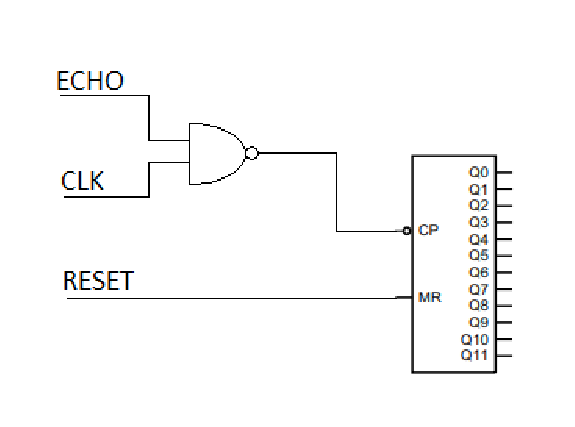
\includegraphics[scale=0.7]{images/COUNTER}
\par\end{centering}
\caption{Counter}
\label{8_7}

\end{figure}

We implemented the NAND before the CP pin to count only when the Echo
is on, and when it becomes off, the counter will stop counting.

\subsubsection{Clock}

The clock was performed also with a NE555 and by following the equation

\[
f=\frac{1}{T}=\frac{1.44}{(R2+2.R1).C3}
\]

we made a clock of the period needed. However, due to the resistor
and capacitor values we had on the university, we only achieved a
\emph{T} of roughly of $80\mu S$ instead of the $100\mu S$ we wanted.
Since it made no such big difference, we left it that way.

\begin{figure}[H]
\begin{centering}
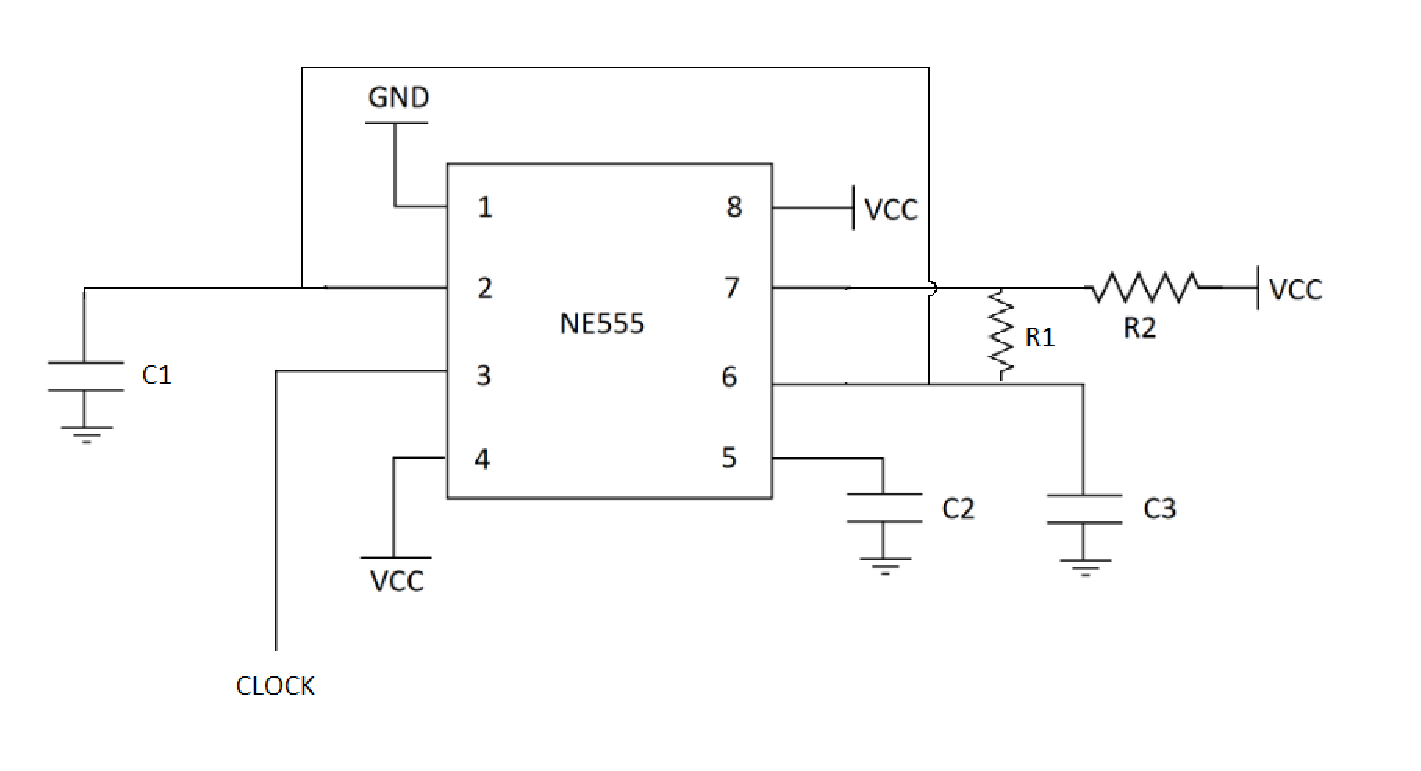
\includegraphics[scale=0.5]{images/CLOCK}
\par\end{centering}
\caption{Clock}

\end{figure}

\paragraph{Visual Output}

Finally for this module, we decided to insert a simple array of LEDs
displaying in binary code the measurement made by the sensor.

\subsection{PCB Fabrication}

To fabricate the design explained before, we used Altium 18 to create
the schematic and design the PCB. Because of the amount of things
taken into account explained before, we decided to implement a double
layer PCB, to make this solution fit in an respectable size. Using
the default library provided by Altium and the LIBEBAL library, we
created the design shown on Figure \ref{8_9}

\begin{figure}[H]
\begin{centering}
\includegraphics[scale=0.7]{\string"images/PCB Layers\string".eps}
\par\end{centering}
\caption{PCB Design}
\label{8_9}
\end{figure}

\begin{figure}[H]
\begin{centering}
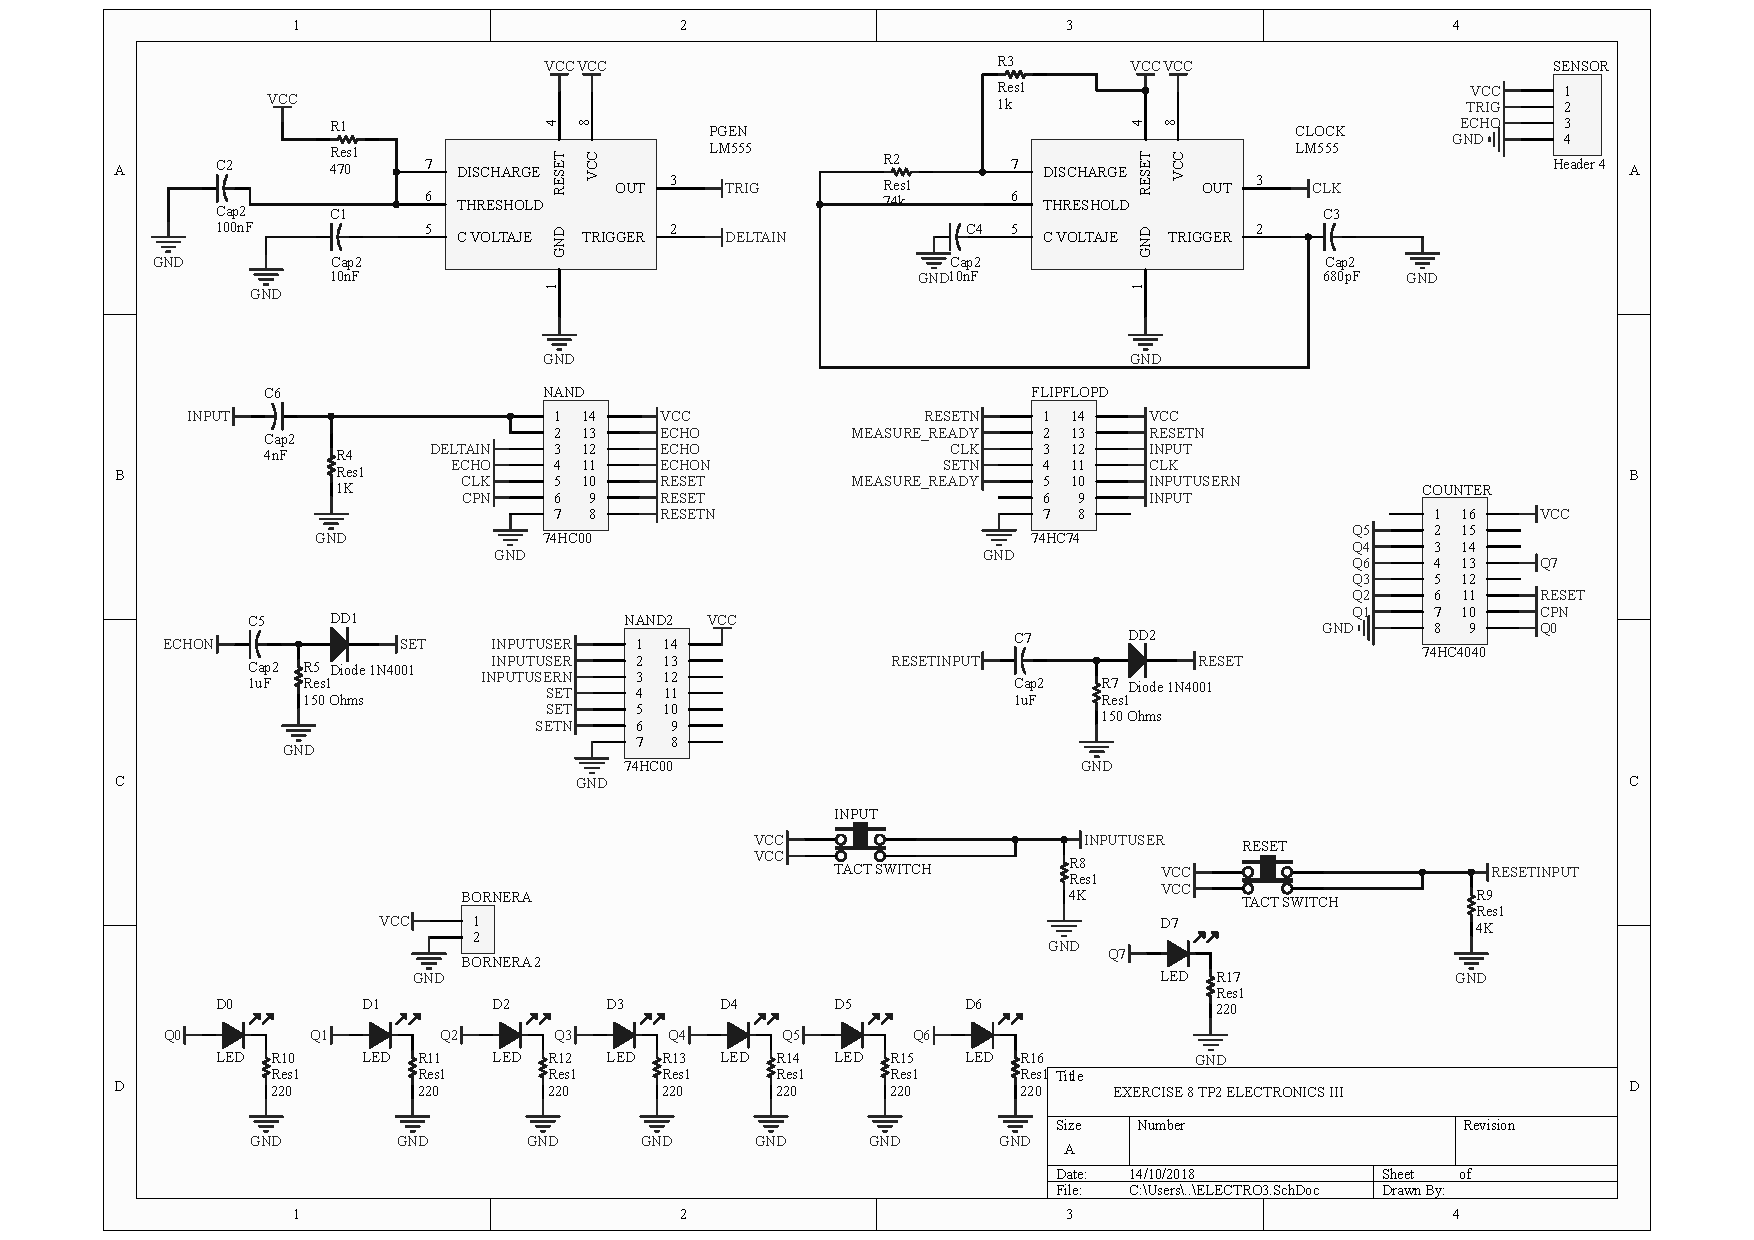
\includegraphics[scale=0.6]{Schematic}
\par\end{centering}
\caption{PCB Schematic}

\end{figure}

\begin{figure}[H]
\begin{centering}
\includegraphics[scale=0.05]{images/TOP}
\par\end{centering}
\caption{PCB Top Layer}

\end{figure}

\begin{figure}[H]
\begin{centering}
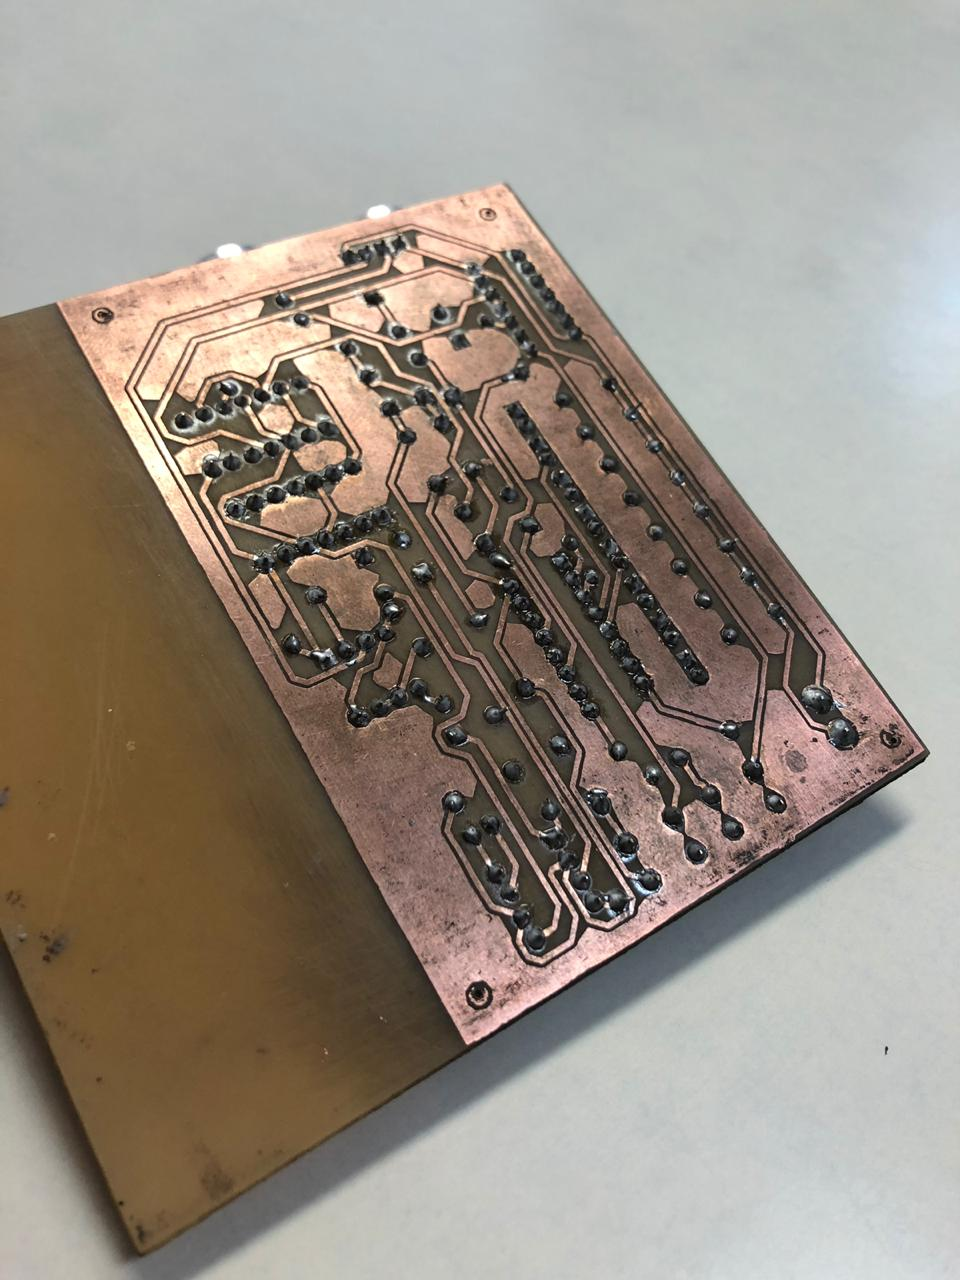
\includegraphics[scale=0.2]{images/BOT}
\par\end{centering}
\caption{PCB Bottom Layer}

\end{figure}

\subsection{Ussage}

To use this solution one simply has to connect the Board to 5V voltage
tension, and press the reset button. Once you are ready to measure,
press the Input Button and a measurement in binary code will be displayed
in the LEDs placed in the PCB. If we call \emph{n} the number in decimal
obtained by the LEDs, we obtain the measurement by following the next
equation

\[
Distance=\frac{n.80}{58}(cm)
\]

Where the number 80 comes from the clock speed and the 58 from the
formula given from the sensor.

\subsection{Conclusions}

We conclude that the Board behaves as expected, and by adjusting the
formula with 80, we can obtain a relatively great measurement of the
distance. Because fabrication and design limitations, we decided not
to add the measure ready LED to display that. This was because to
human perspective, the measurement is practically instant and adding
2 more components to the PCB was not enough gain to make the trouble.
However, the Board to our perspective works perfectly.
